Neste capítulo apresentam-se e analisam-se os resultados obtidos após se ter seguido a
metodologia explicada no capítulo anterior. Descreve-se os resultados após a
eliminação de \textit{outliers}, mostram-se os histogramas e gráficos de barra obtidos para
cada um dos atributos e os resultados do coeficiente de correlação de Kendall para a
relação entre variáveis. 

\section{Eliminação de Outliers}
Conforme dito anteriormente, a análise de quais alunos são \textit{outliers} foi feita
estudando caso a caso os alunos que não conseguiram passar em nenhuma disciplina.
Caso se constatasse que o aluno não tinha conseguido passar por ter abandonado a
universidade, o aluno era tratado como outlier e seus dados eram removidos do espaço
amostral. Eliminaram-se 203 estudantes do espaço amostral dessa maneira, ficando-se
assim com 3751 amostras. 

\section{Histogramas e Gráficos de Barra Para Atributos}
Apresentam-se a seguir os histograms e gráficos de barra para os atributos que puderam
ser calculados. Como alguns atributos dependiam de informação acerca da quantidade de
créditos de cada matéria, e não tinha-se tal informação disponível no começo da
pesquisa, não foi possível gerar a estatística descritiva para tais atributos. Tais
atributos são descritos mais adiante, na seção \ref{atributos_problematicos}.

\subsection{Gráfico de Barra para Atributo Sexo}
A Figura \ref{atr_sex} mostra o gráfico de barra para o atributo sexo. O gráfico
está de acordo com o esperado, quando se leva em conta que a presença de mulheres em
curso de exatas ainda é, lamentavelmente, restrita. 
\begin{figure}[!ht]
    \caption{Gráfico de Barra para Atributo Sexo}
    \centering
    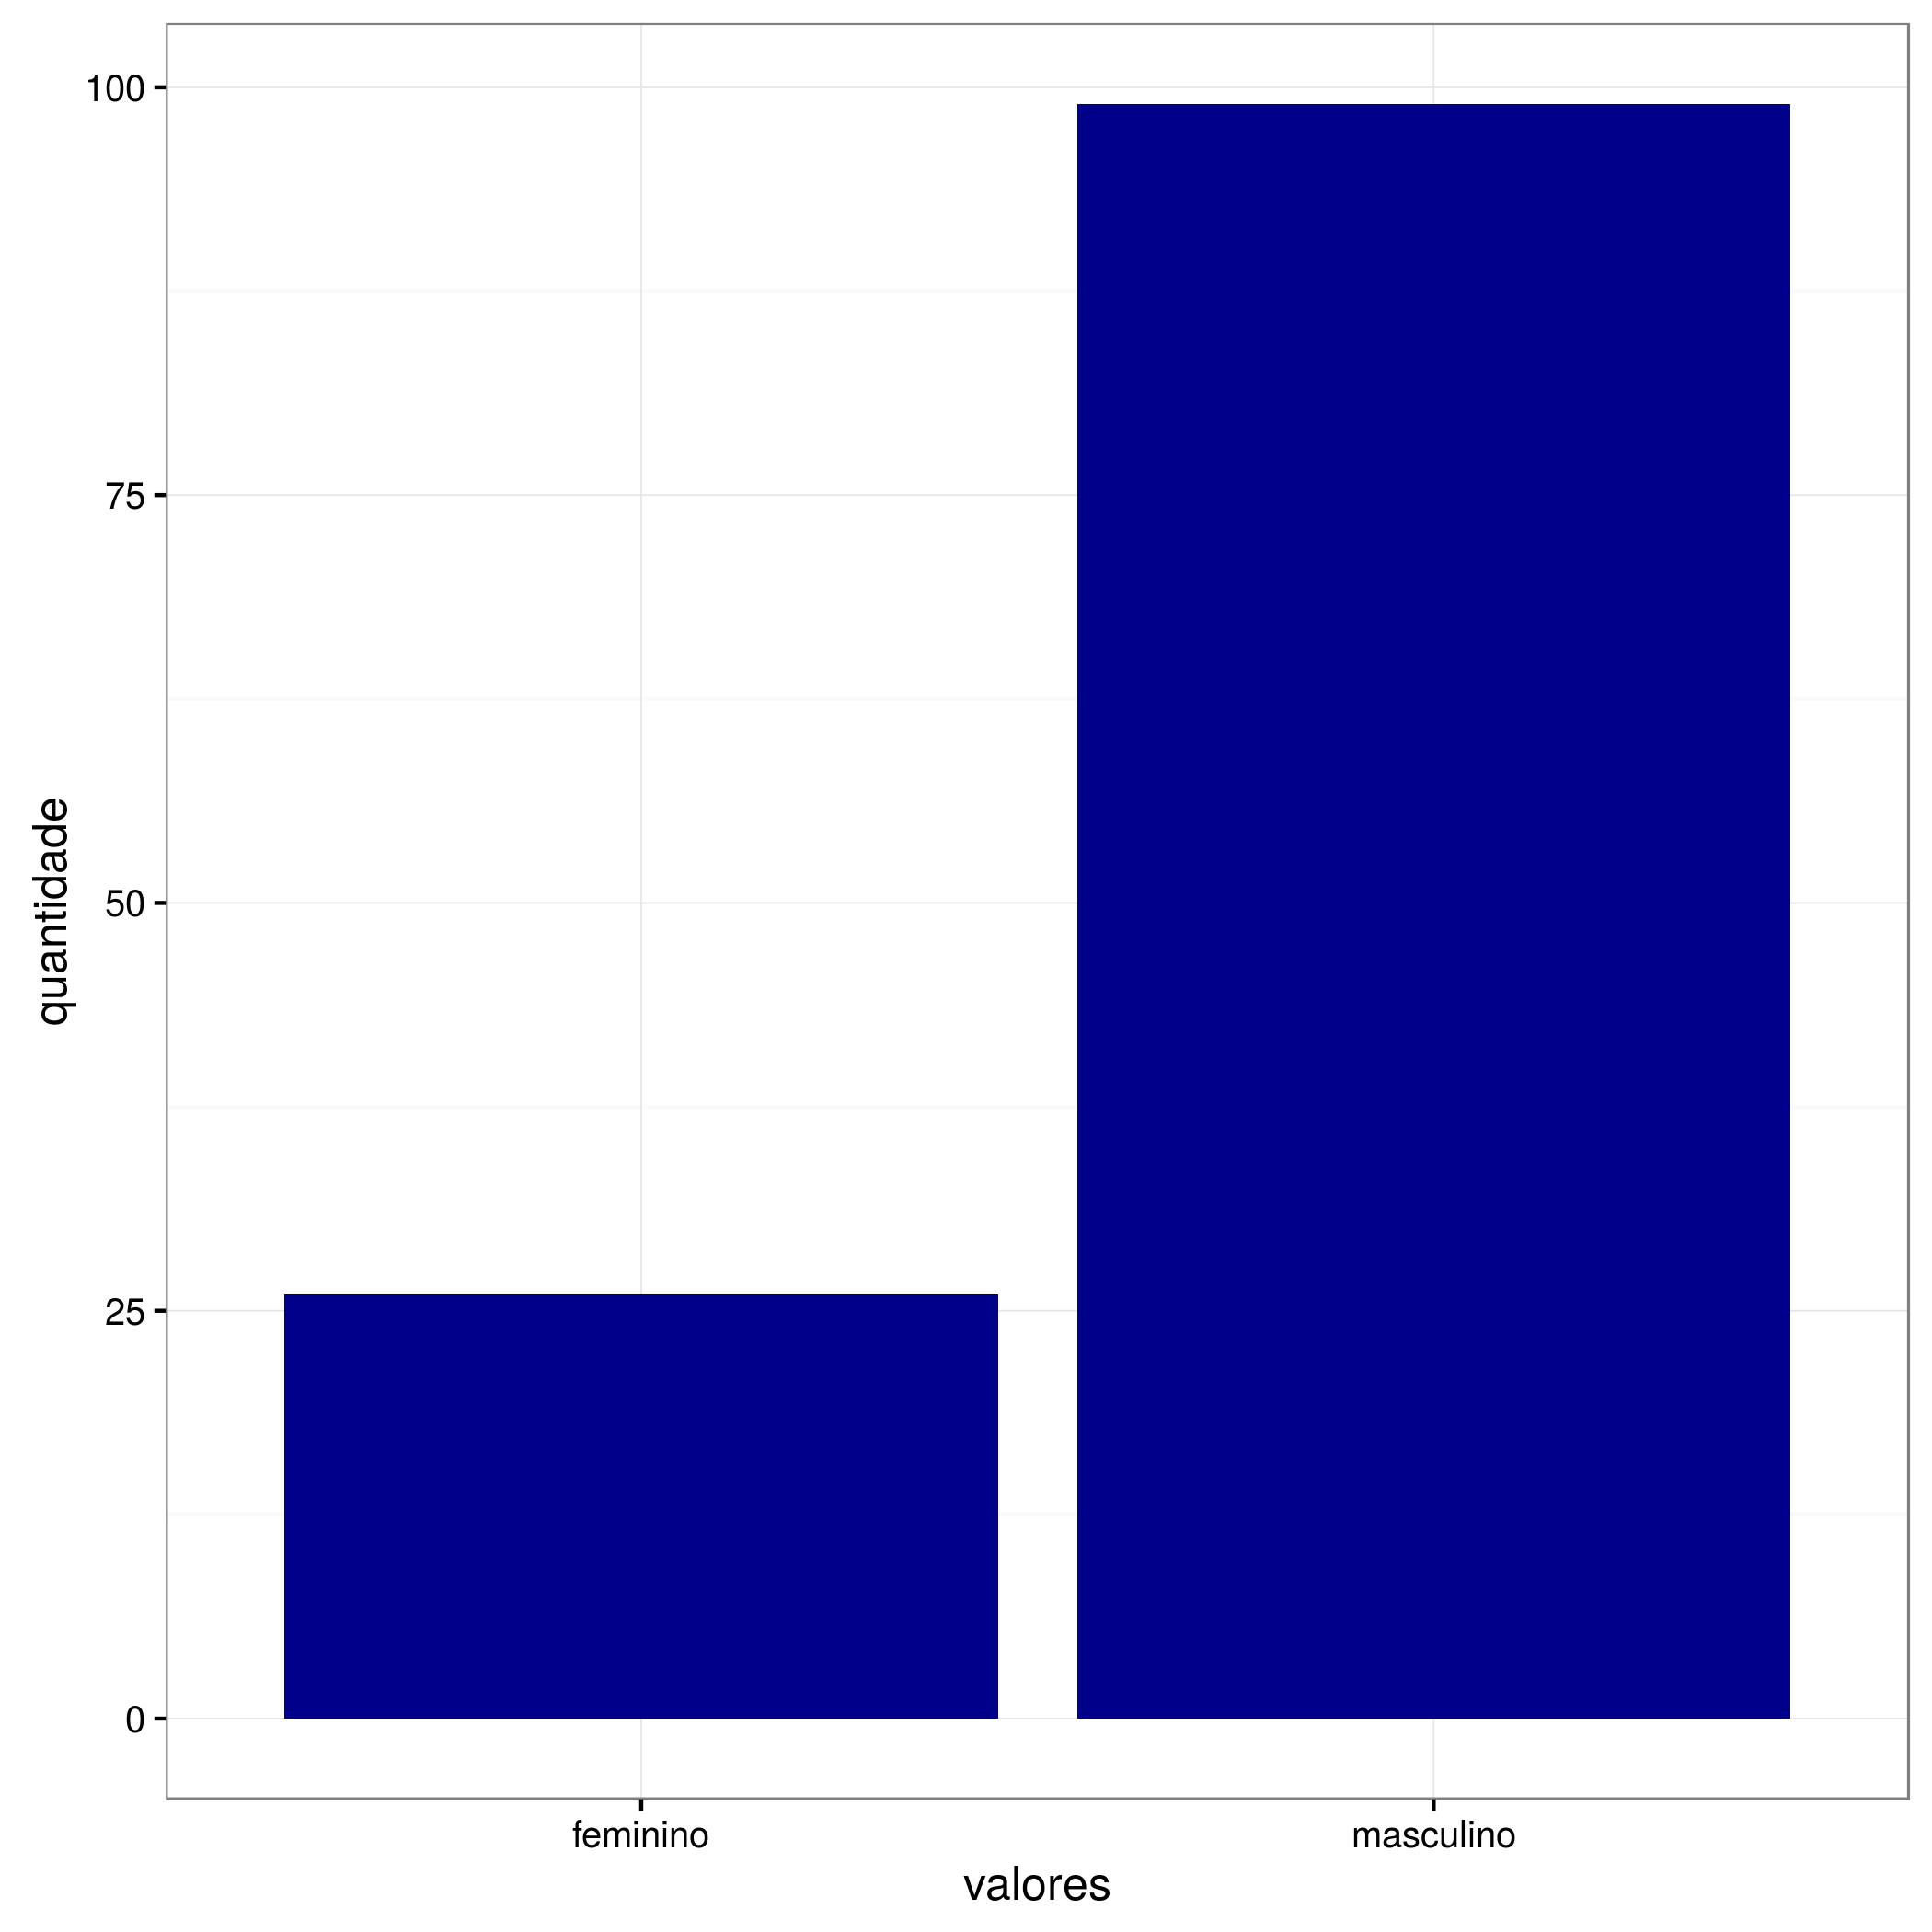
\includegraphics[width = 10cm]{sex.png}
    \label{atr_sex}
\end{figure}

\subsection{Gráfico de Barra para Atributo Idade}
A Figura \ref{atr_age} mostra o gráfico de barra para o atributo idade. O gráfico
mostra que os ingressantes na UnB têm idade em torno dos 18/19 anos. 
\begin{figure}[!ht]
    \caption{Gráfico de Barra para Atributo Idade}
    \centering
    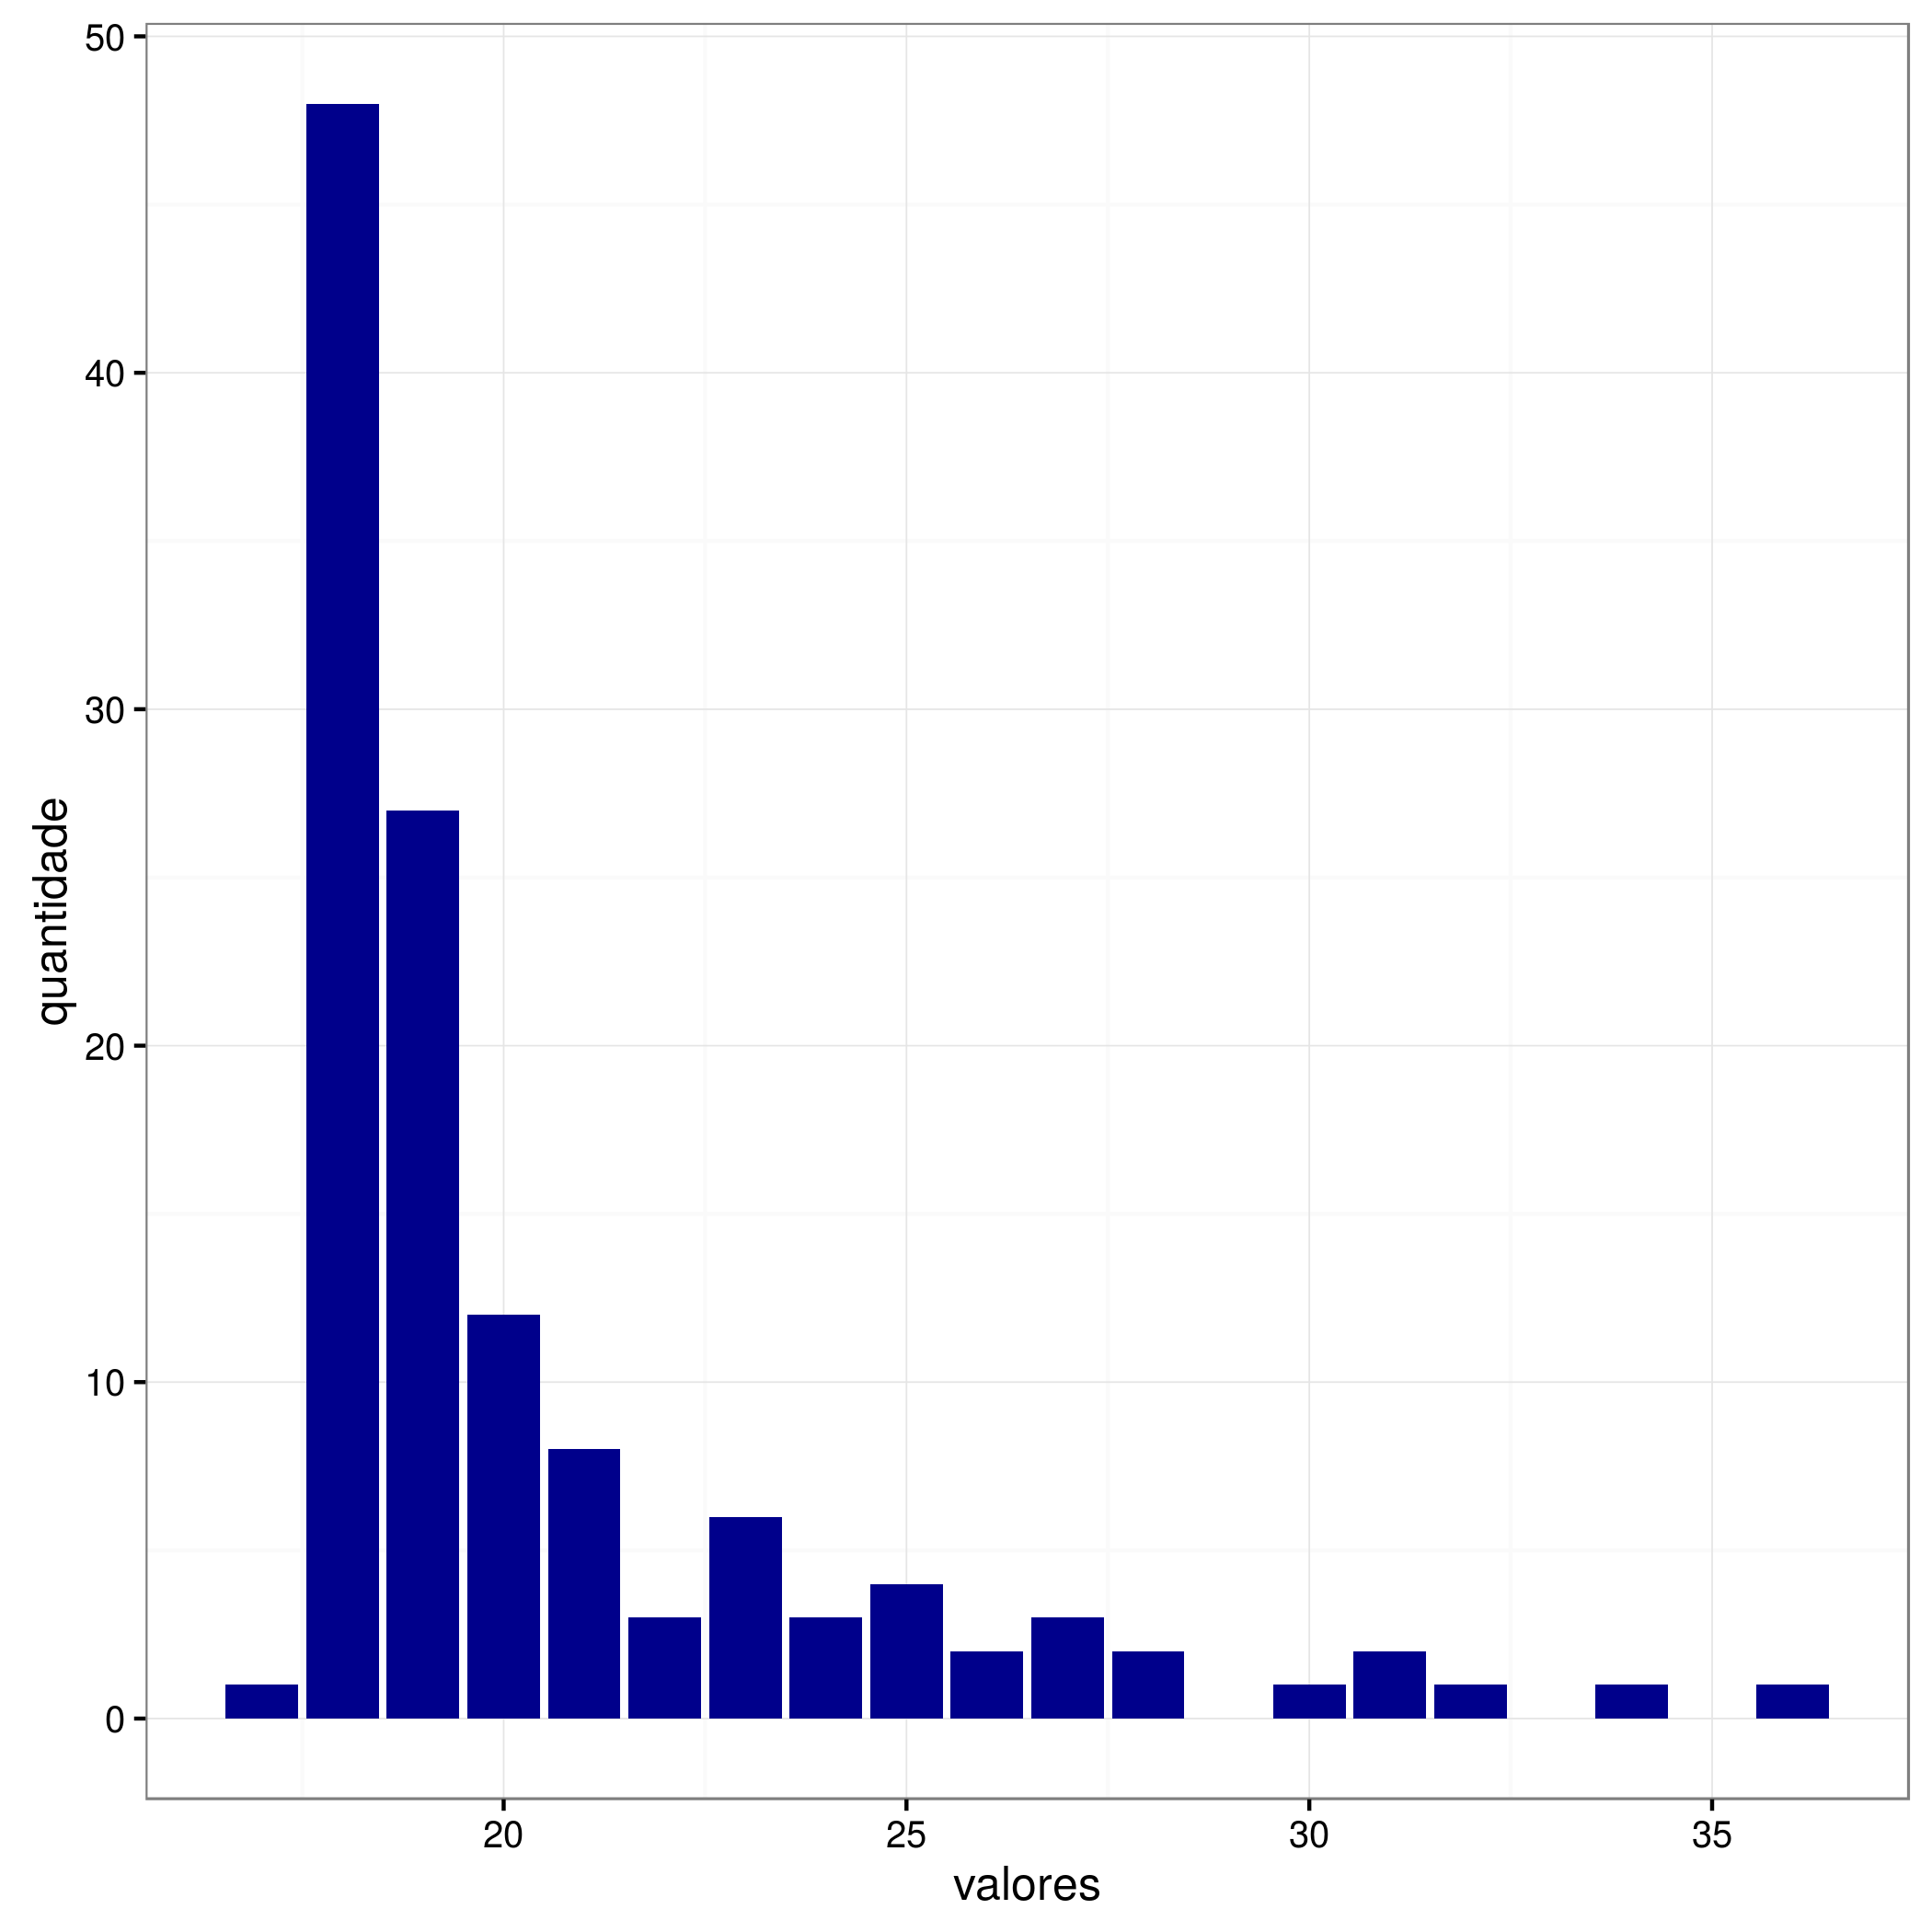
\includegraphics[width = 10cm]{age.png}
    \label{atr_age}
\end{figure}

\subsection{Gráfico de Barra para Atributo Residência}
A Figura \ref{atr_res} mostra o gráfico de barra para o atributo residência. Pode-se
notar que nesse caso a quantidade de valores faltantes (barra com nome
\texttt{indisponível} é pequena). 
\begin{figure}[!ht]
    \caption{Gráfico de Barra para Atributo Residência}
    \centering
    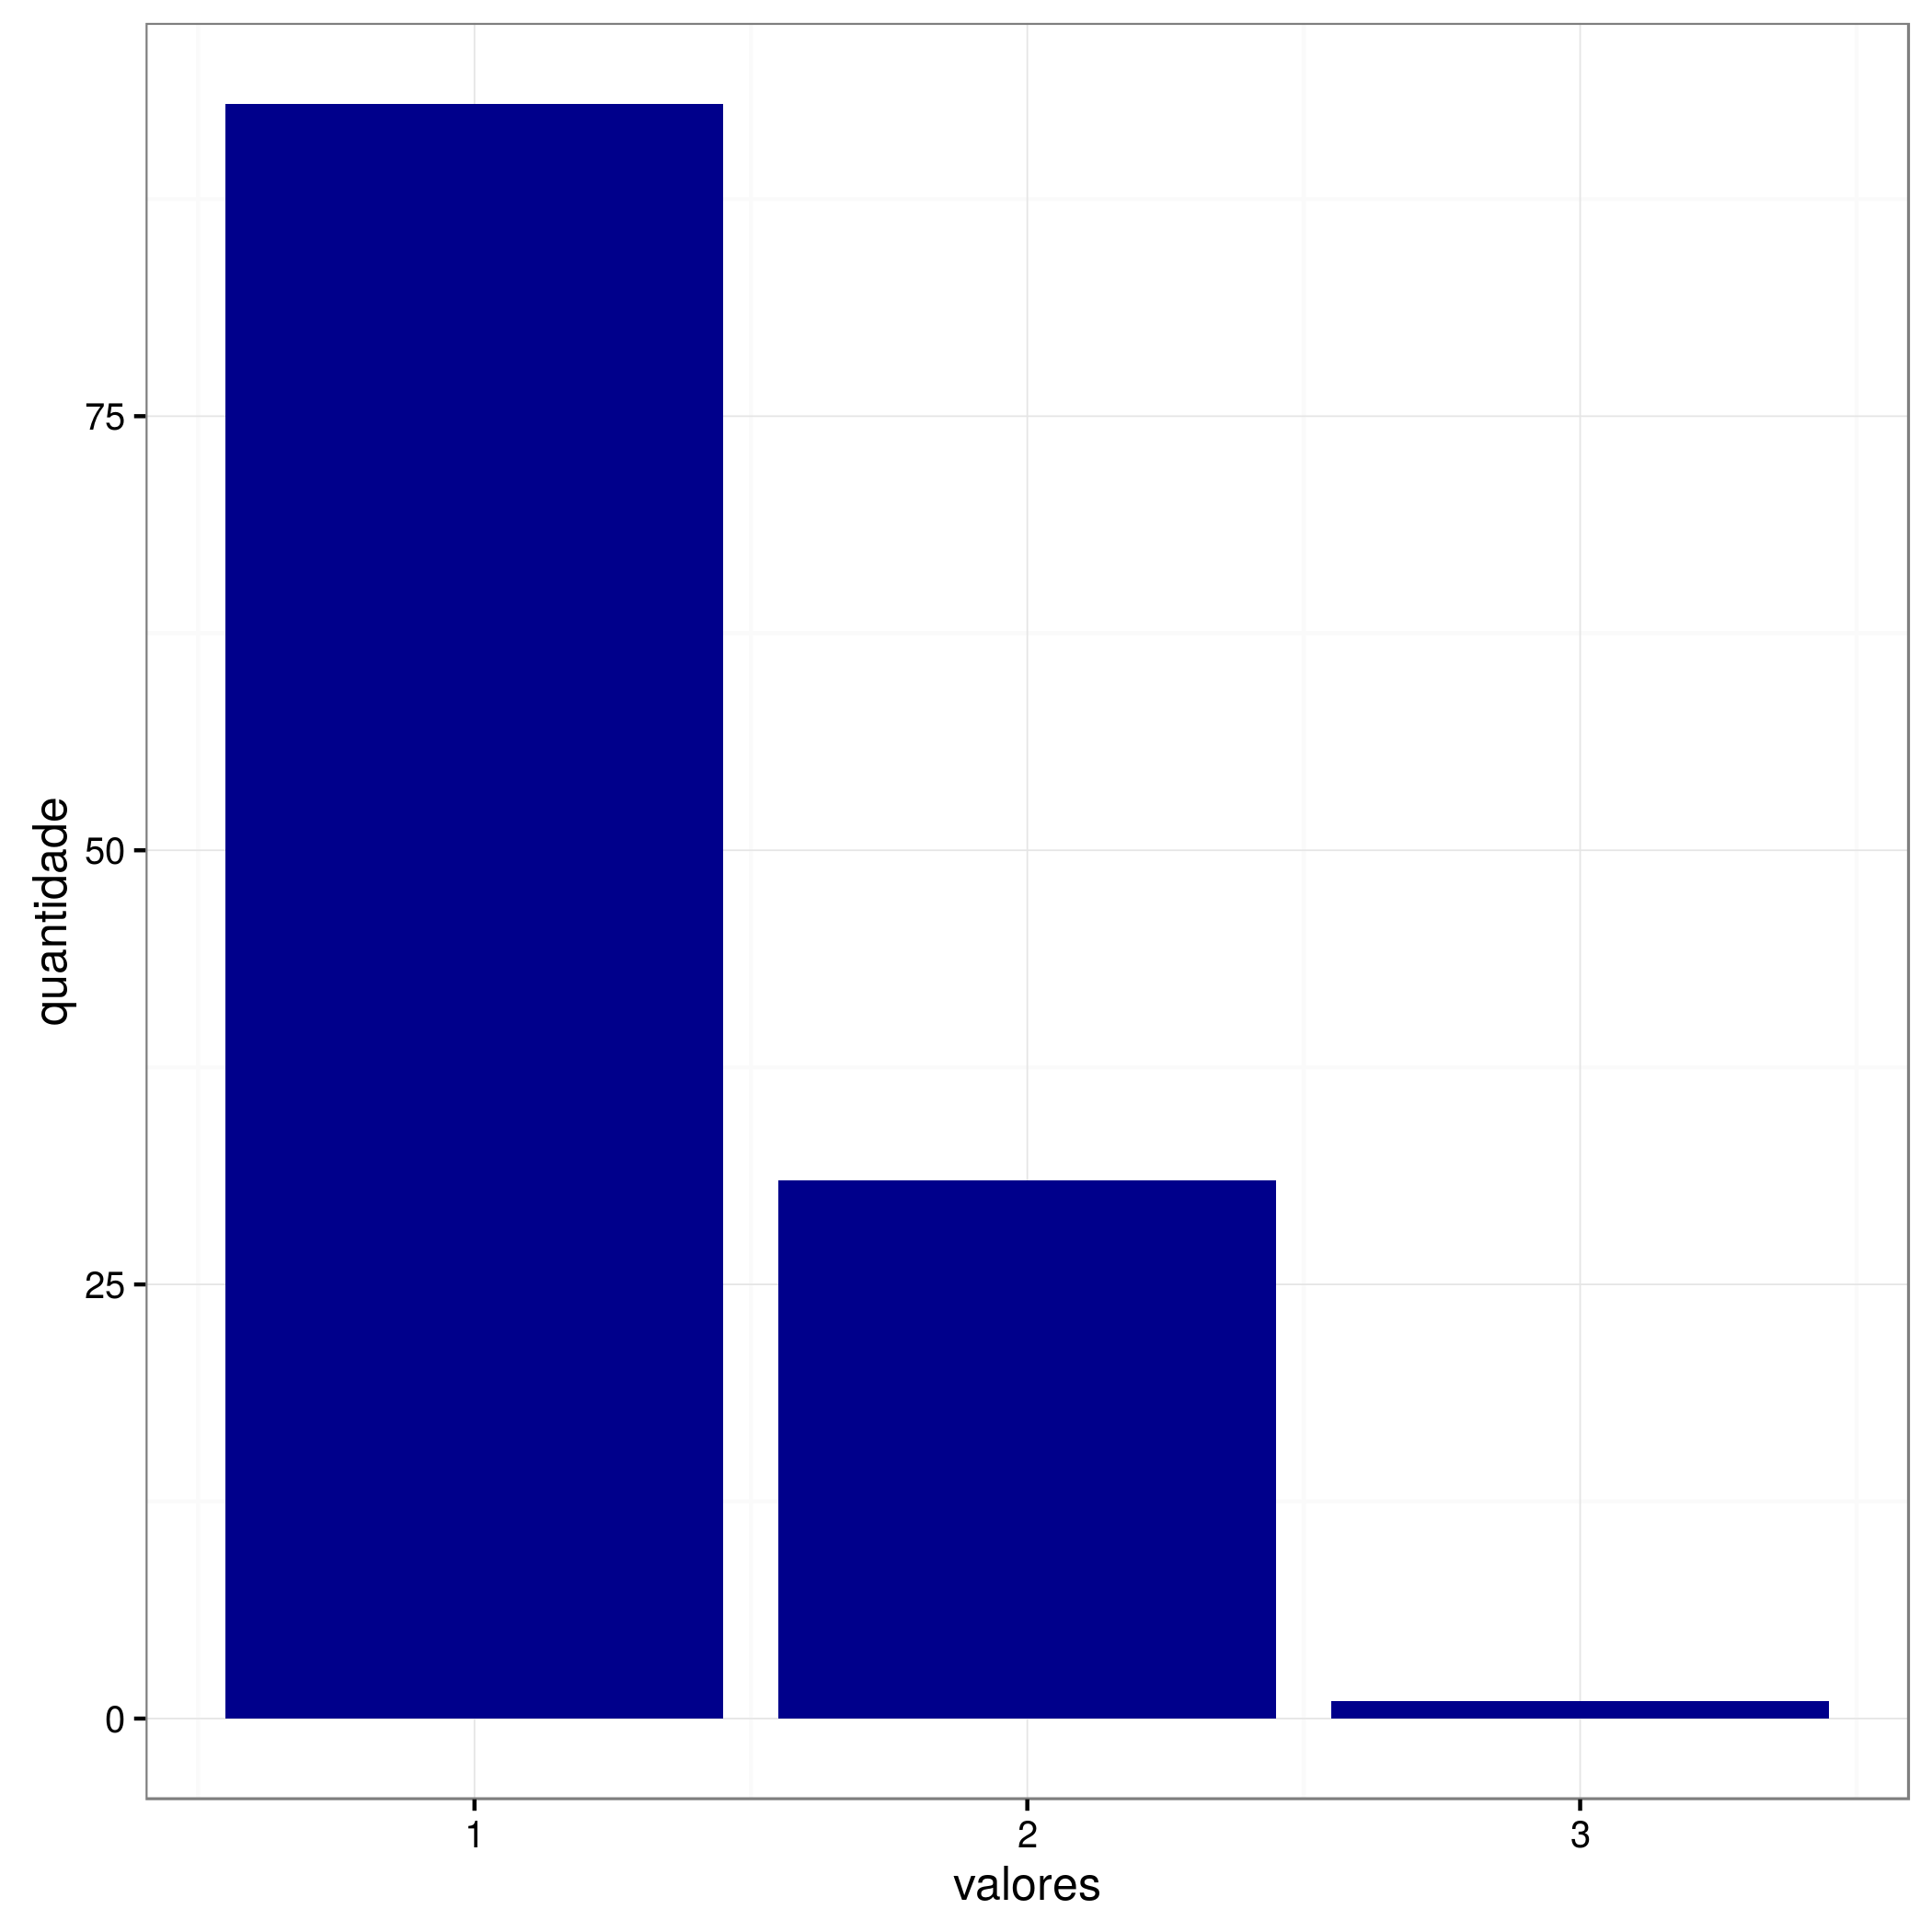
\includegraphics[width = 10cm]{local.png}
    \label{atr_res}
\end{figure}
\clearpage

\subsection{Gráfico de Barra para Atributo Cota}
A Figura \ref{atr_quota} mostra o gráfico de barra para o atributo cota. 
\begin{figure}[!ht]
    \caption{Gráfico de Barra para Atributo Cota}
    \centering
    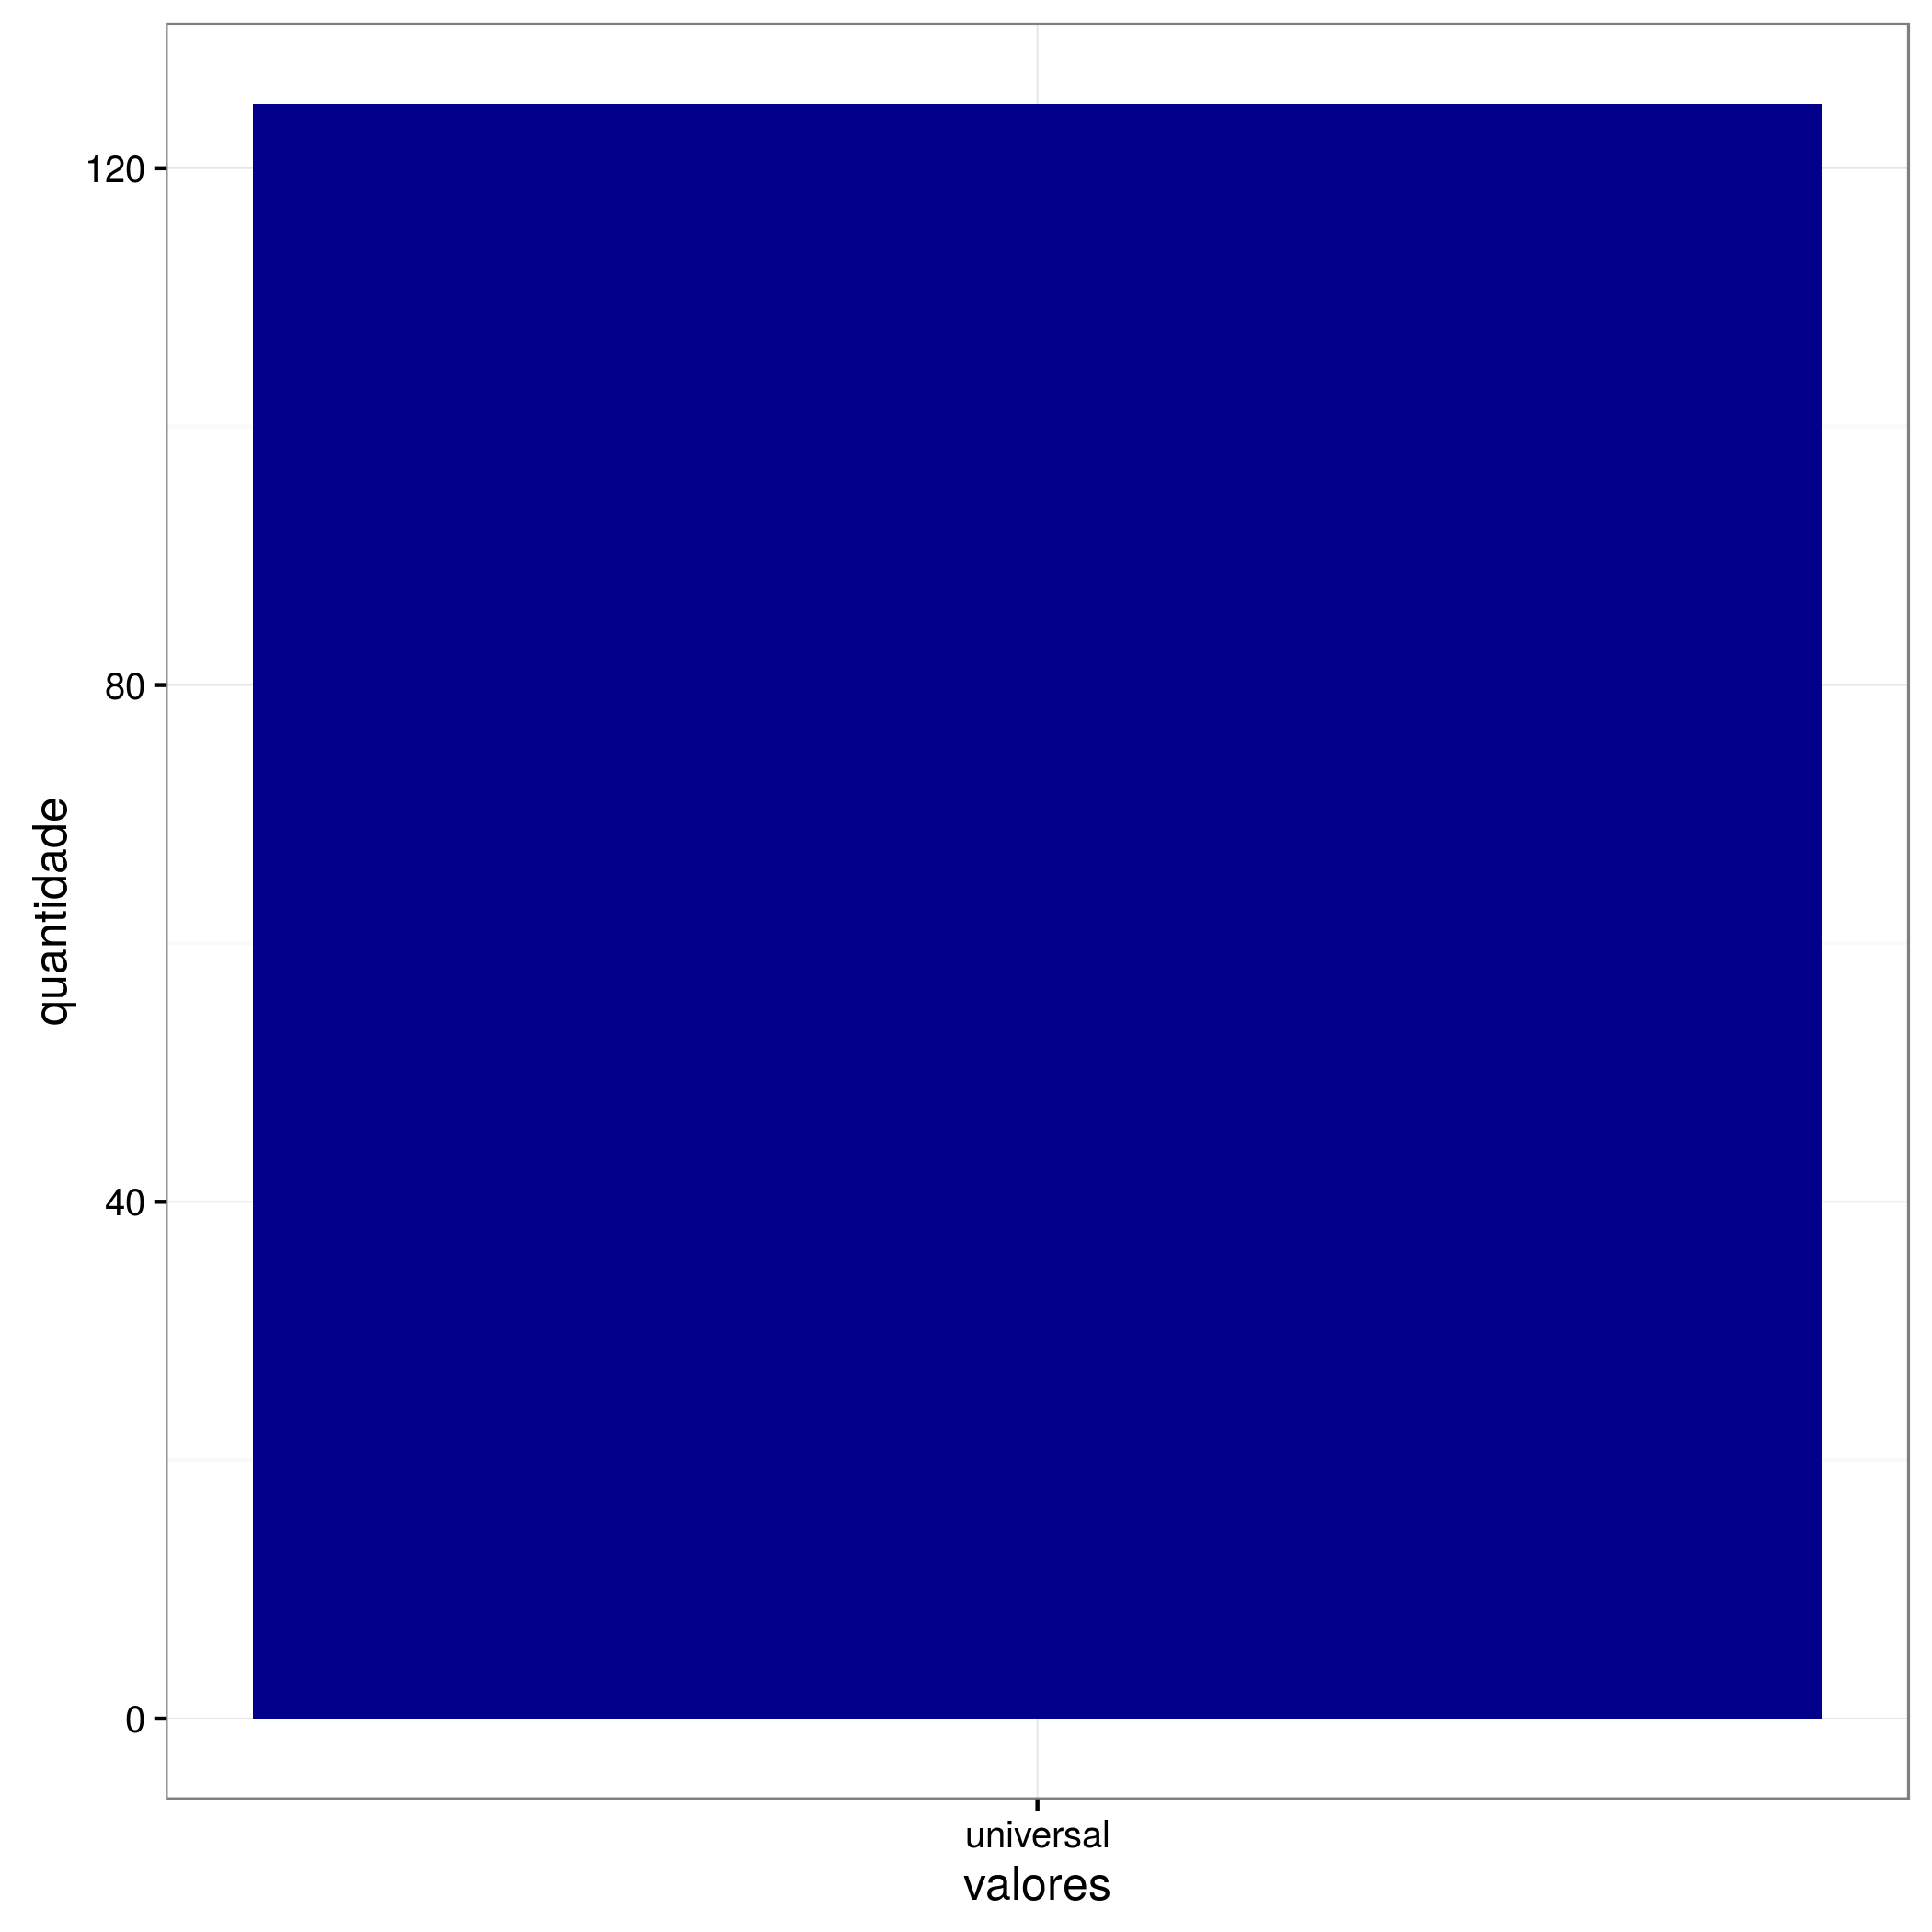
\includegraphics[width = 10cm]{quota.png}
    \label{atr_quota}
\end{figure}

Por questões de legibilidade, a legenda no gráfico foi encurtada. Seu significado é
apresentado a seguir: 
\begin{itemize}
    \item \texttt{negro}: Detentor de cotas para negros.
    \item \texttt{p\_alta\_nppi}: Detentor de cotas para alunos de escola pública de
        alta renda que não é preto, pardo ou indígena.
    \item \texttt{p\_alta\_ppi}: Detentor de cotas para alunos de escola pública de
        alta renda que é preto, pardo ou indígena.
    \item \texttt{p\_baixa\_ppi}: Detentor de cotas para alunos de escola pública de
        baixa renda que é preto, pardo ou indígena.
    \item \texttt{p\_baixa\_nppi}: Detentor de cotas para alunos de escola pública de
        baixa renda que não é preto, pardo ou indígena.
    \item \texttt{universal}: Não detém cotas.
\end{itemize}

\subsection{Gráfico de Barra para Atributo Tipo da Escola}
A Figura \ref{atr_school} mostra o gráfico de barra para o atributo tipo da escola.
Pode-se notar que a presença de valores faltantes é significativa. Apesar disso,
decidiu-se manter esse atributo em nosso estudo. 
\begin{figure}[!ht]
    \caption{Gráfico de Barra para Atributo Tipo da Escola}
    \centering
    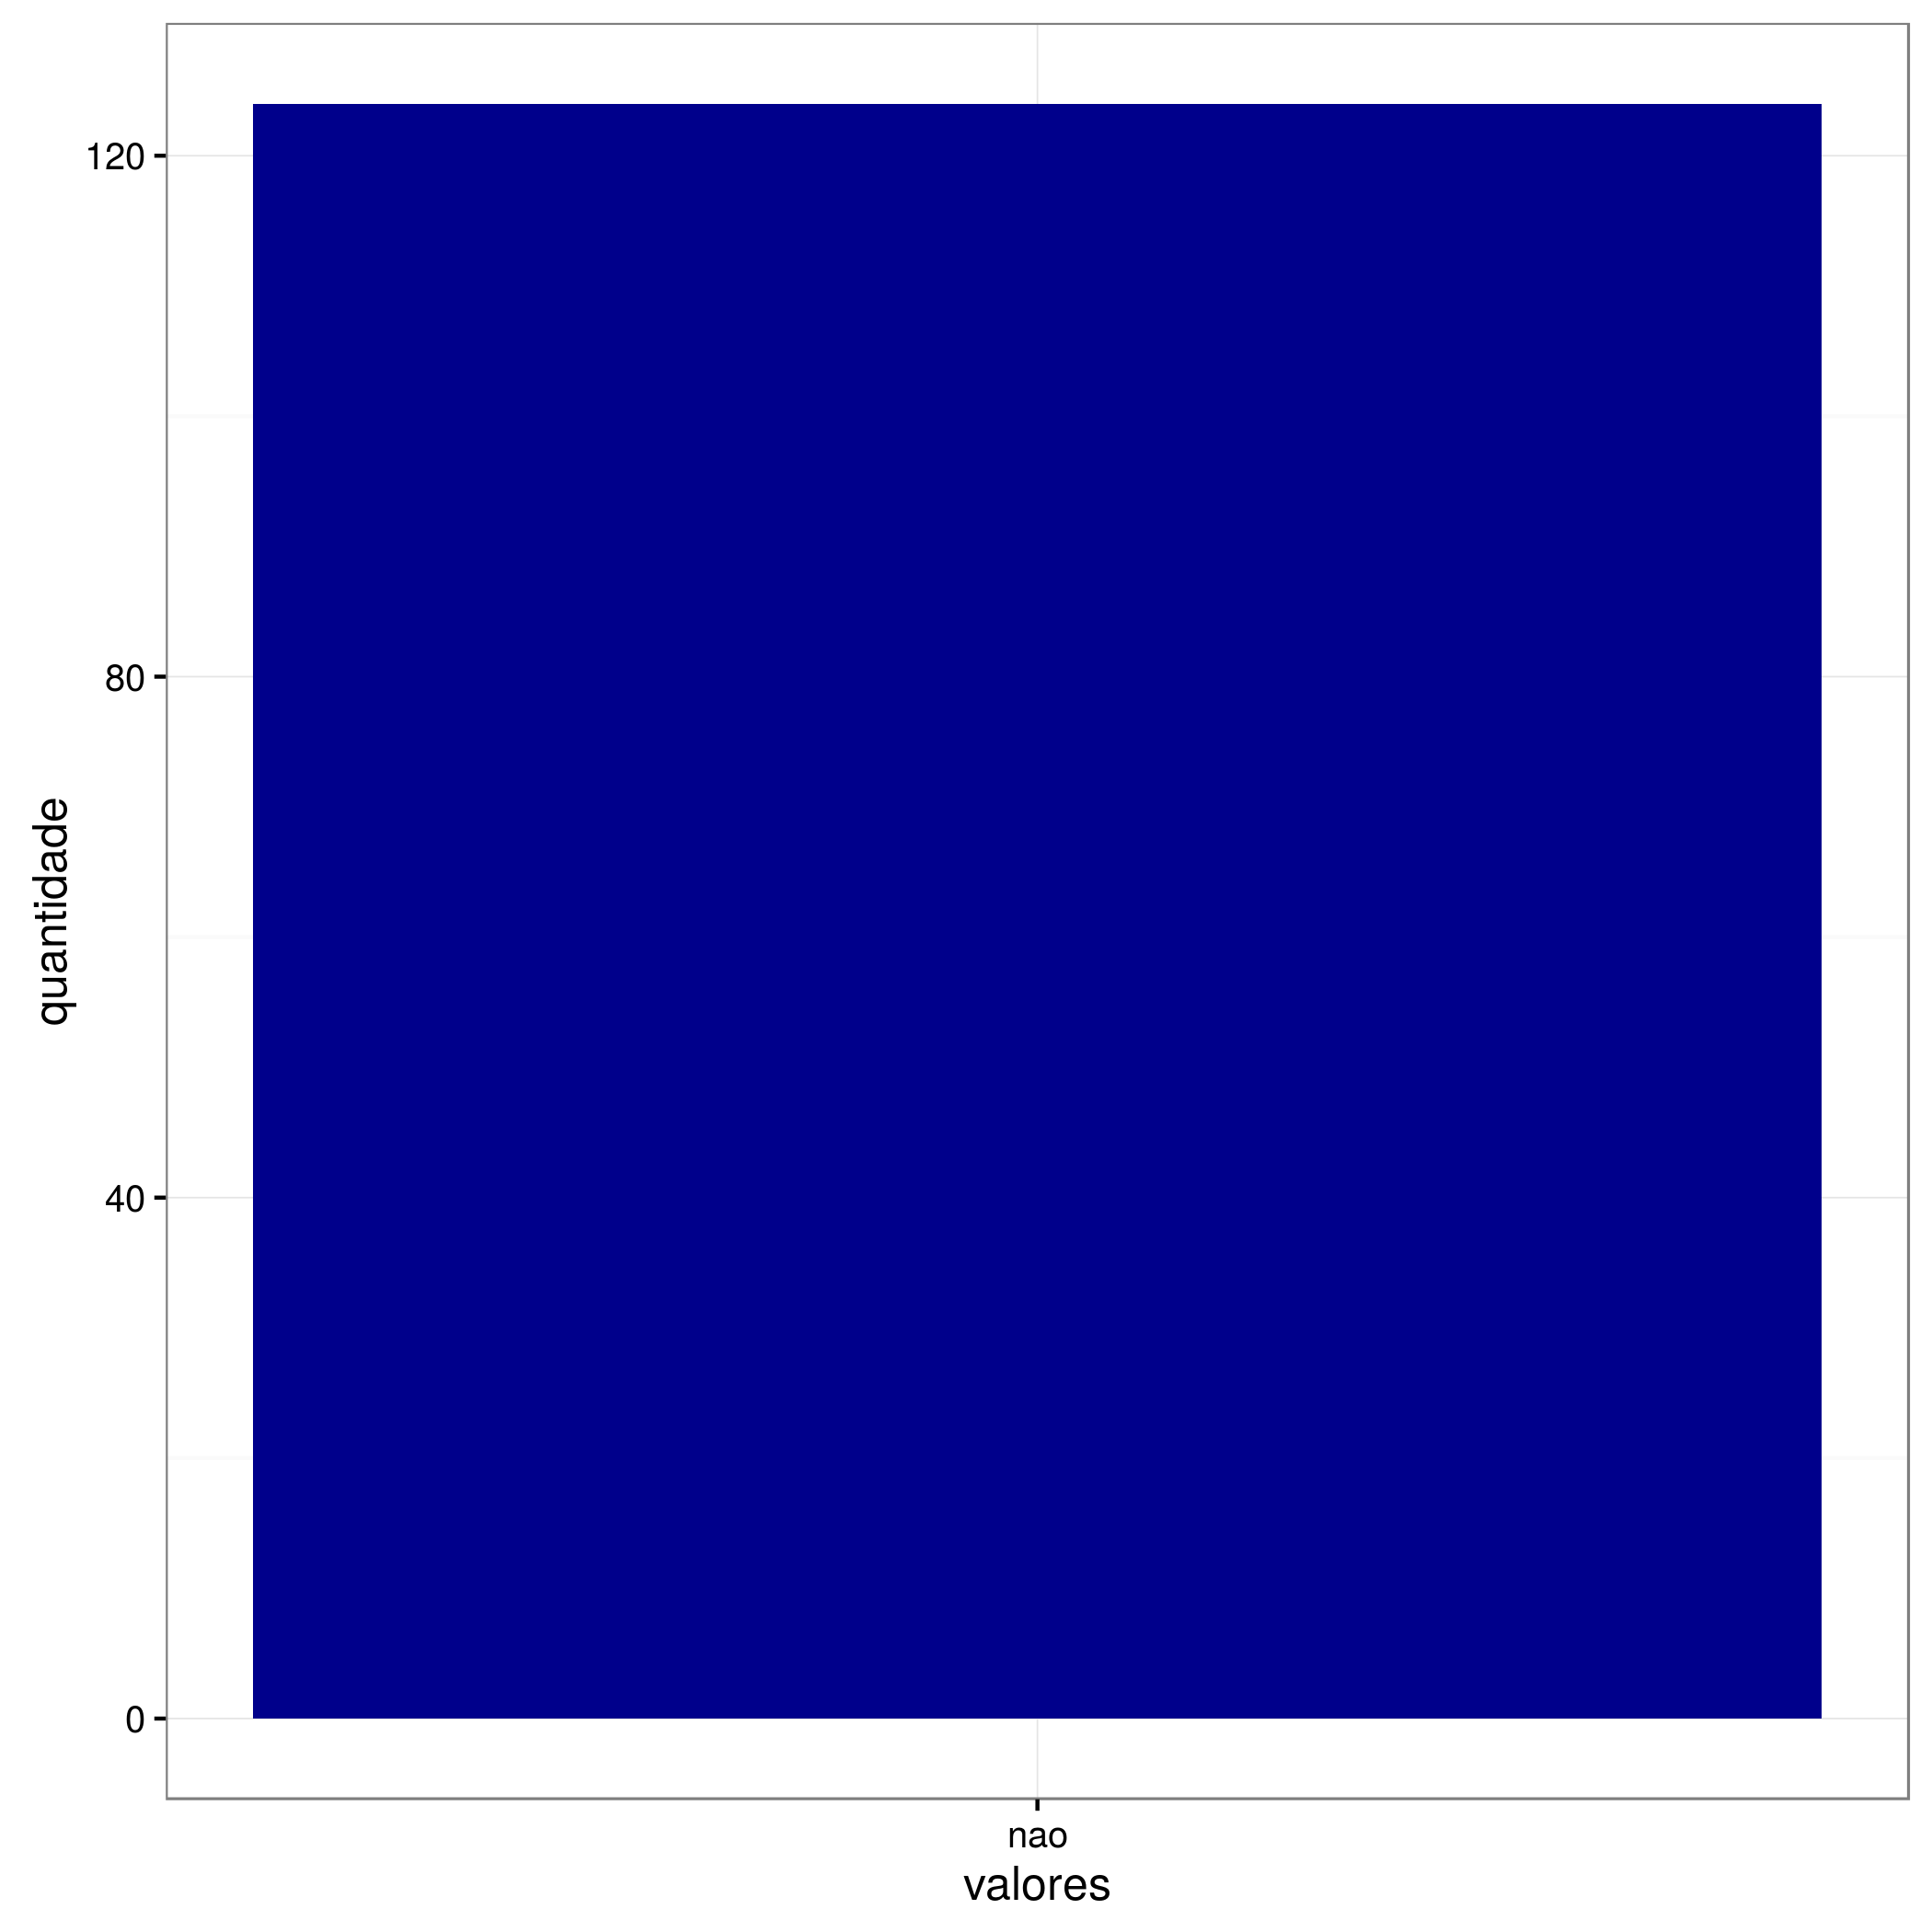
\includegraphics[width = 10cm]{school_type.png}
    \label{atr_school}
\end{figure}

\subsection{Gráfico de Barra para Atributo Curso}
A Figura \ref{atr_course} mostra o gráfico de barra para o atributo curso. 

\begin{figure}[!ht]
    \caption{Gráfico de Barra para Atributo Curso}
    \centering
    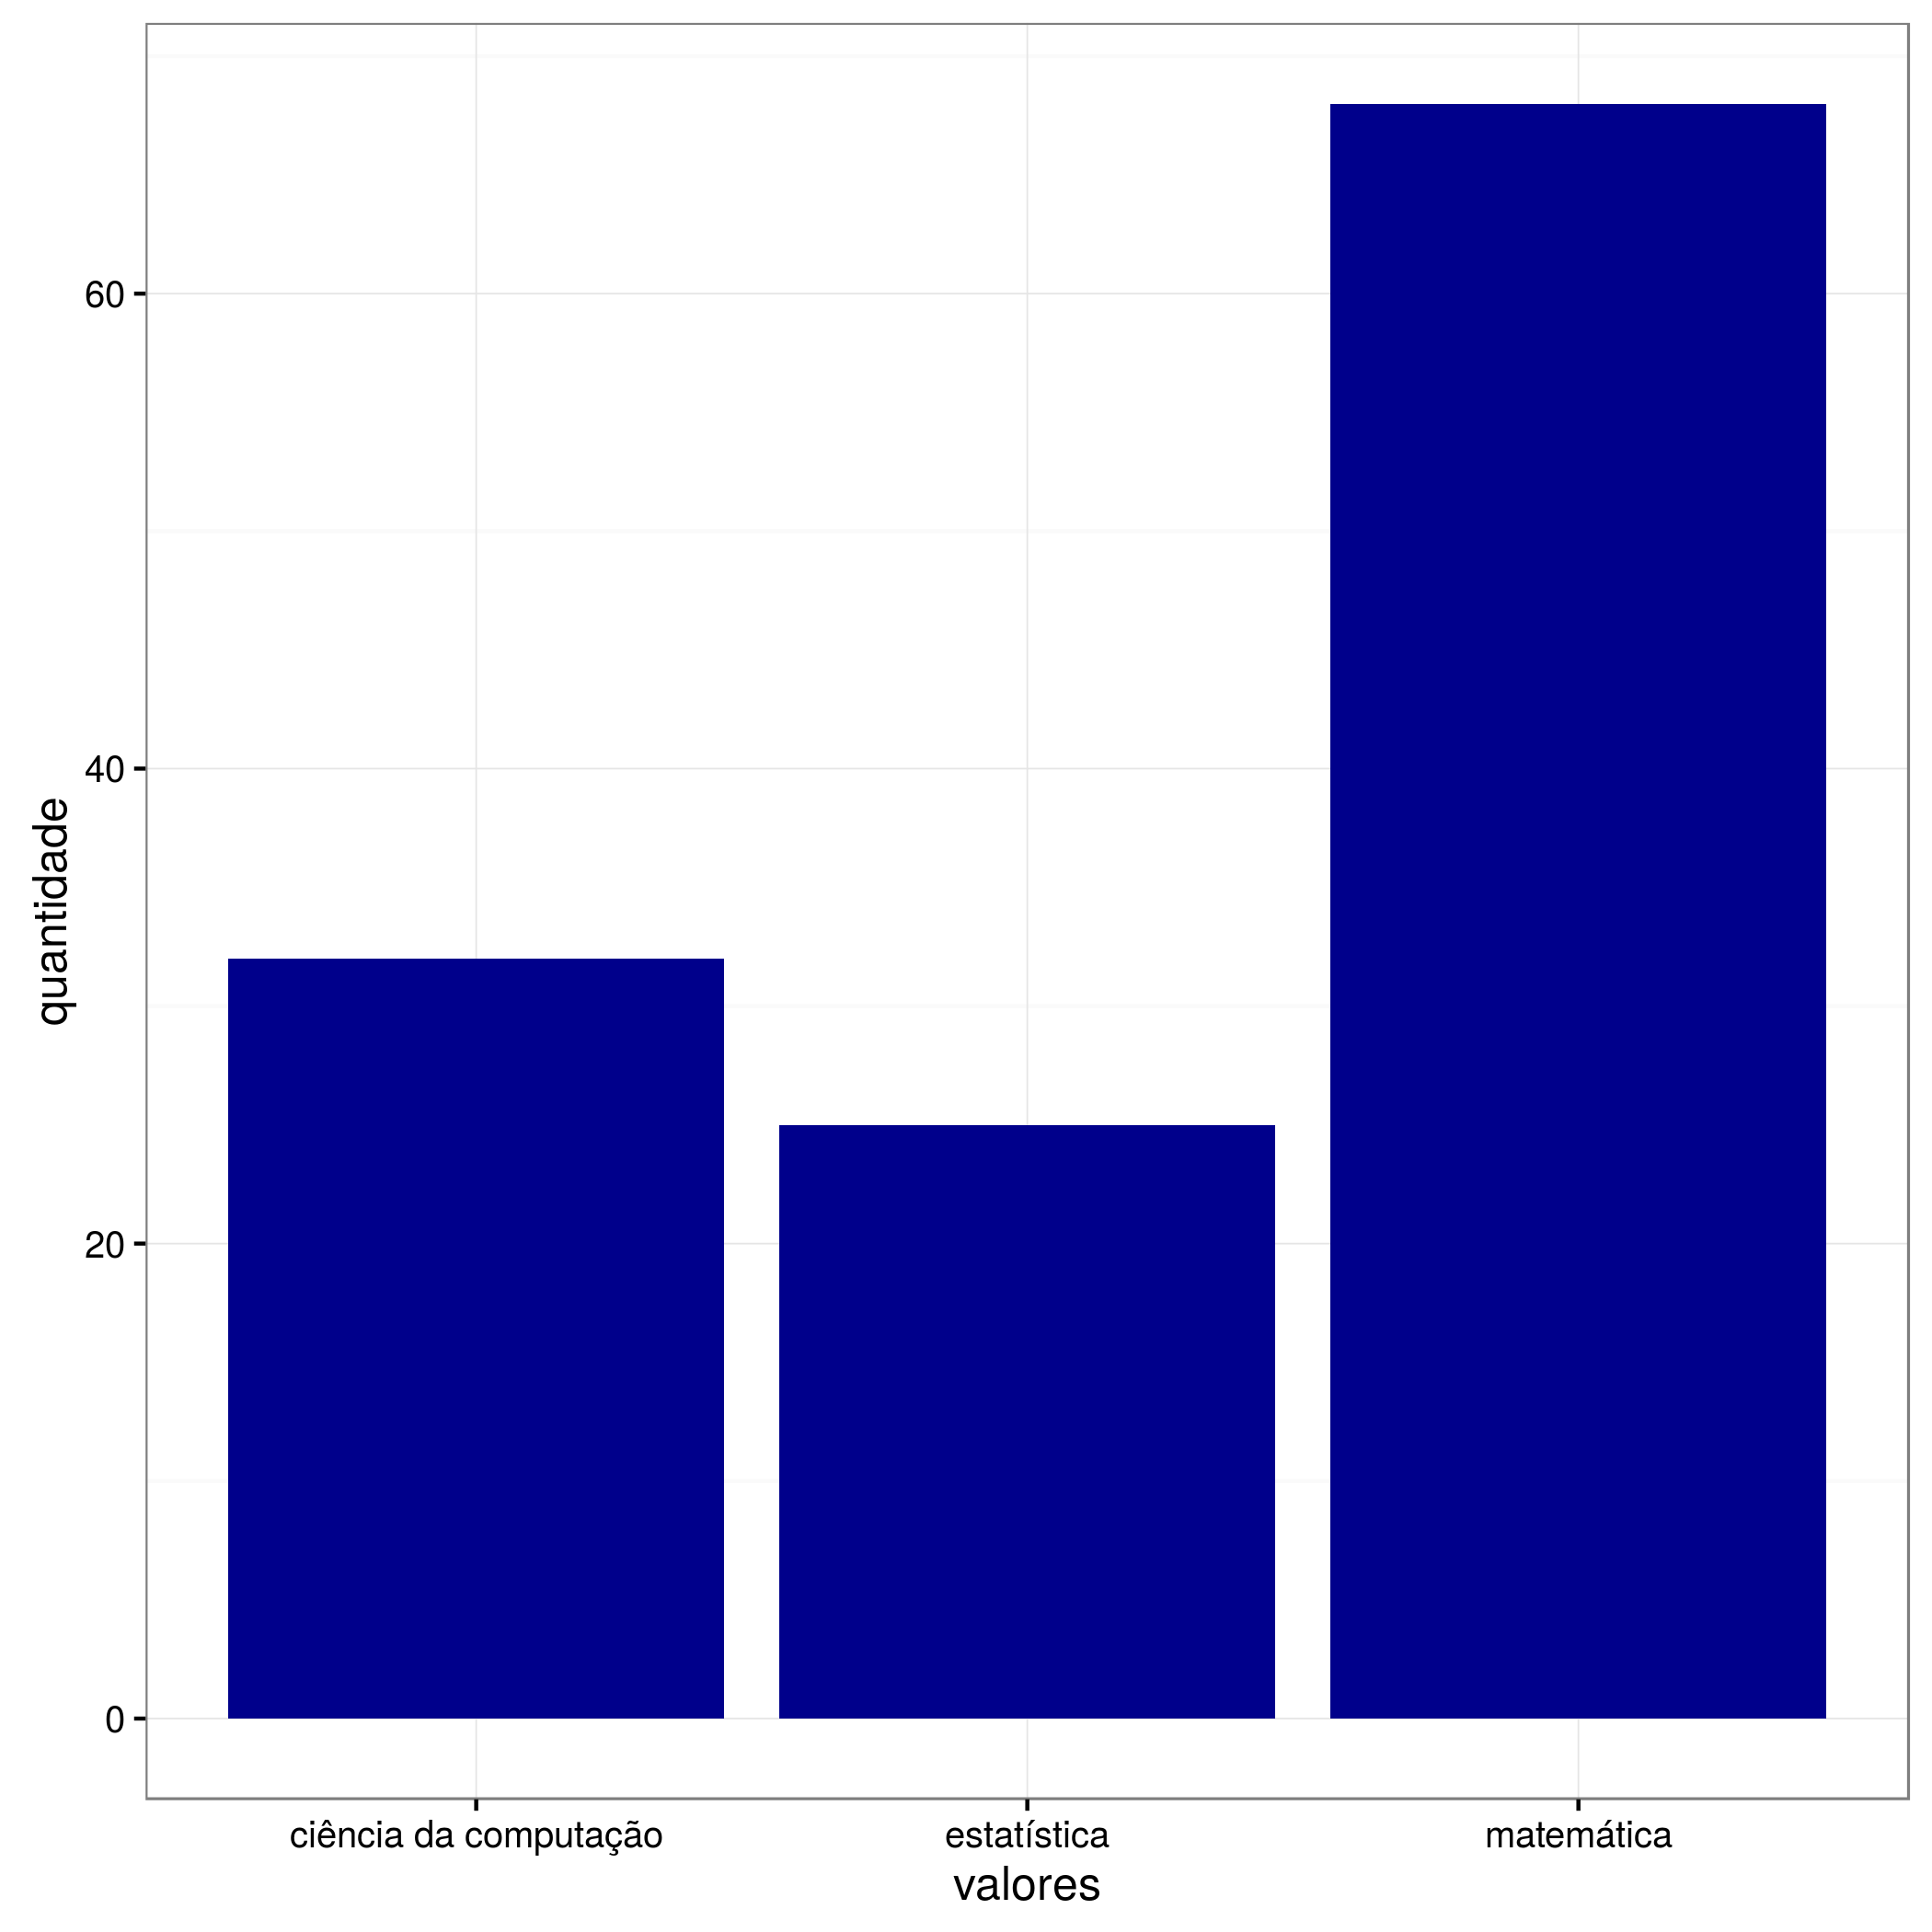
\includegraphics[width = 10cm]{course.png}
    \label{atr_course}
\end{figure}

Por questões de legibilidade, a legenda no gráfico foi encurtada. Seu significado é
apresentado a seguir: 
\begin{itemize}
    \item \texttt{cic\_b}: Alunos de Ciência da Computação (Bacharelado).
    \item \texttt{cic\_lic}: Alunos de Ciência da Computação (Licenciatura).
    \item \texttt{eng\_comp}: Alunos de Engenharia da Computação.
    \item \texttt{eng\_mec}: Alunos de Engenharia Mecatrônica.
    \item \texttt{eng\_redes}: Alunos de Engenharia de Redes. 
    \item \texttt{eng\_softw}: Alunos de Engenharia de Software
\end{itemize}

%TODO: se quiser encher linguiça, falar tb que redes e mecatrônica são mais recentes
%tb. 
Pode-se notar que os cursos de engenharia da computação e engenharia de software
apresentam muito menos alunos que os demais. Isso se deve ao fato de tais cursos
terem tido início após o período considerado na pesquisa. 
\clearpage

\subsection{Gráfico de Barra para Atributo Raça}
A Figura \ref{atr_race} mostra o gráfico de barra para o atributo raça. 
\begin{figure}[!ht]
    \caption{Gráfico de Barra para Atributo Raça}
    \centering
    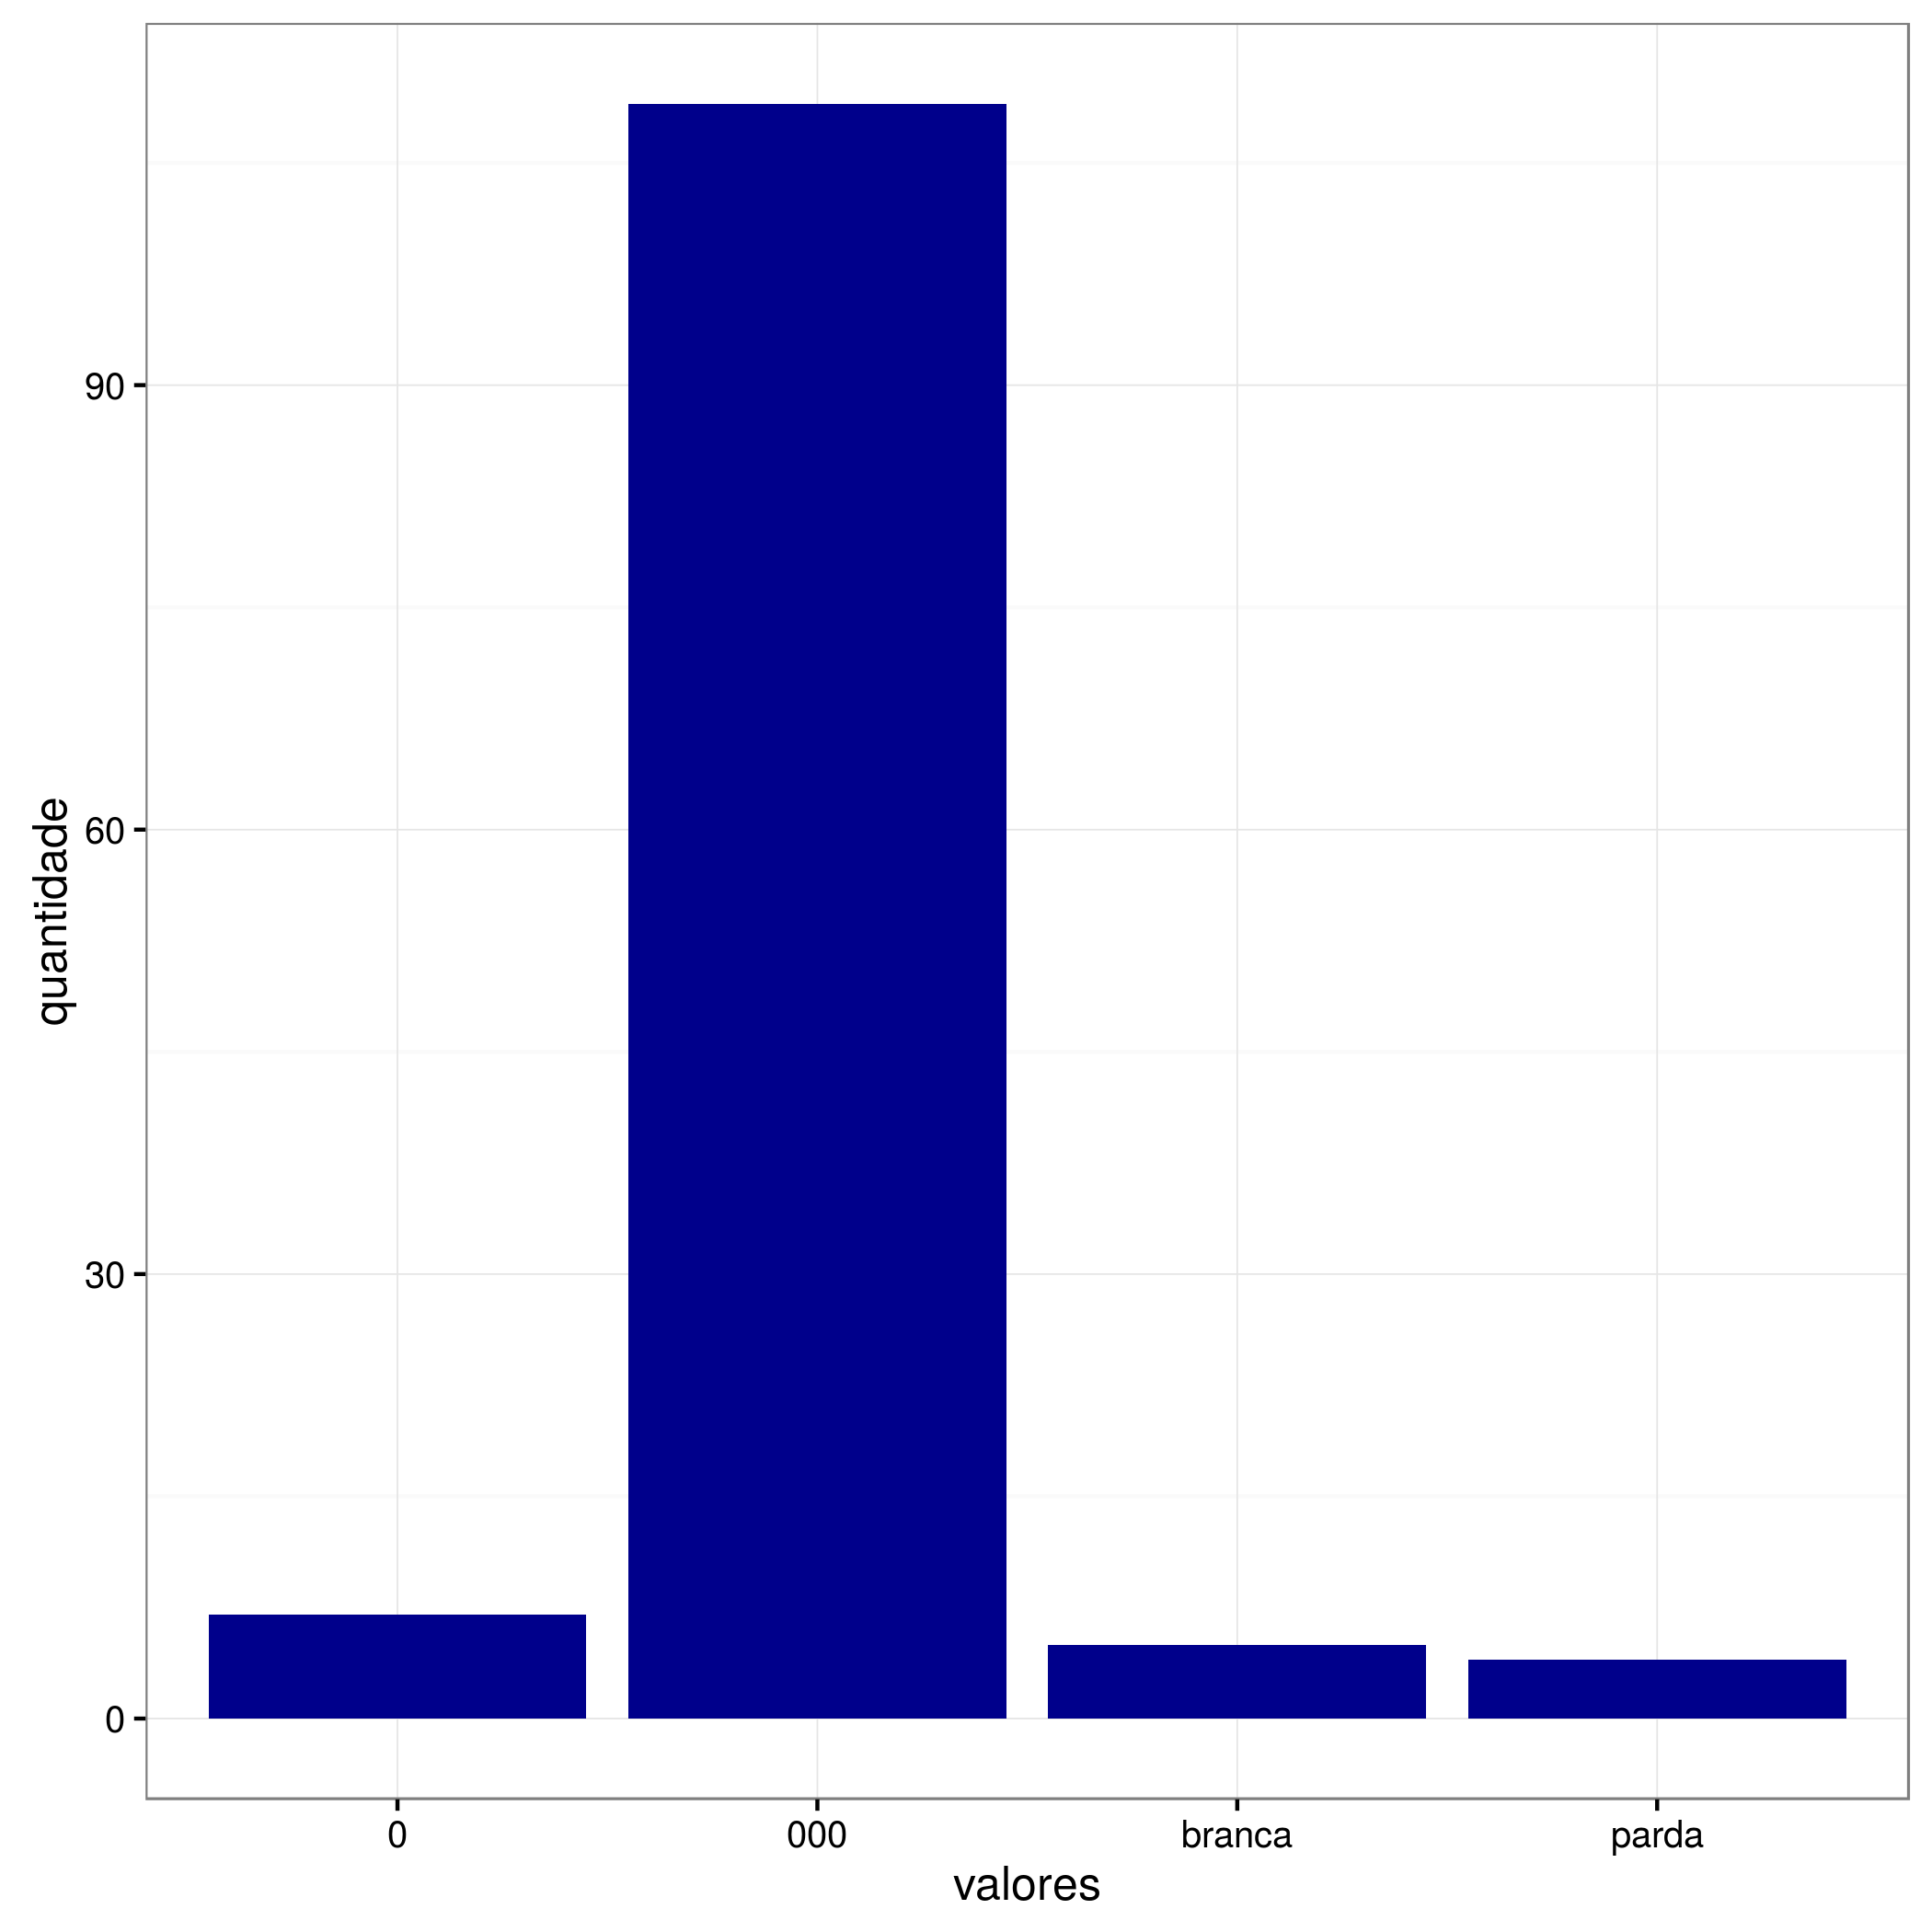
\includegraphics[width = 10cm]{race.png}
    \label{atr_race}
\end{figure}
Pode-se observar que há uma grande quantidade de valores faltantes, de modo que
optou-se por tirar esse atributo de análises posteriores. 

\subsection{Análise para Atributo Forma de Ingresso}
A Figura \ref{atr_way_in} mostra o gráfico de barra para o atributo forma de ingresso. 
Por questões de legibilidade, a legenda no gráfico foi encurtada. Seu significado é
apresentado a seguir: 
\begin{itemize}
    \item \texttt{vest}: Ingresso via Vestibular
    \item \texttt{ci}: Ingresso via Convênio-Int
    \item \texttt{to}: Ingresso via Transferência Obrigatória
    \item \texttt{to}: Ingresso via Transferência Obrigatória
    \item \texttt{ac}: Ingresso via Acordo Cultural PEC
    \item \texttt{ca}: Ingresso via Convênio Andifes
    \item \texttt{mc}: Ingresso via Matrícula Cortesia
    \item \texttt{tf}: Ingresso via Transferência Facultativa
    \item \texttt{ppp}: Ingresso via PEC-G Peppfol
    \item \texttt{pdcs}: Ingresso pois é portador de diploma de curso superior
    \item \texttt{vmc}: Ingresso via Vestibular para Mesmo Curso
\end{itemize}

\begin{figure}[!ht]
    \caption{Gráfico de Barra para Atributo Forma de Ingresso}
    \centering
    \includegraphics[width = 10cm]{way_in.png}
    \label{atr_way_in}
\end{figure}

Seguindo a isso, fez-se a análise da quantidade de alunos em cada categoria. Os
valores são mostrados na Tabela \ref{tab_way_in}.

% todo: por tabela
\begin{table}
\begin{center}
\begin{tabular}[c]{| c | c | c | c |}
    \hline
    Forma de Ingresso & Total de Alunos & Alunos Formados & Porcentagem \\
    \hline
    Vestibular & 2695 & 1176 & 44\% \\
    \hline
    Convênio Andifes & 7 & 0 & 0\% \\
    \hline
    Acordo Cultural-PEC & 8 & 4 & 50\% \\
    \hline
    Portador de Diploma de Curso Superior & 17 & 0 & 0\% \\
    \hline
    Transferência Facultativa & 40 & 16 & 40\% \\
    \hline
    Matrícula Cortesia & 35 & 4 & 11\% \\
    \hline
    Convênio Int & 17 & 0 & 0\% \\
    \hline
    SISU & 25 & 0 & 0\% \\
    \hline
    Transferência Obrigatória & 104 & 23 & 22\% \\
    \hline
    PAS & 794 & 392 & 49\% \\
    \hline
    Vestibular para Mesmo Curso & 1 & 0 & 0\% \\
    \hline
\end{tabular}
\end{center}
\caption{Para cada forma de ingresso mostram-se o número de alunos que
entraram, a quantidade que foi capaz de se formar e a qual a porcentagem representada
por estes.}
\label{tab_way_in}
\end{table}

Os resultados mostram que alguns poucos alunos entraram por algumas formas de
ingresso. Diante disso, optou-se por trabalhar com o atributo categórico forma de
ingresso considerando apenas as opções: PAS, Vestibular, Transferência e Outros. 
 
\subsection{Gráfico de Barra para Atributo Forma de Saída}
A Figura \ref{atr_way_out} mostra o gráfico de barra para o atributo forma de saída. 
Por questões de legibilidade, a legenda no gráfico foi encurtada. Seu significado é
apresentado a seguir: 
\begin{itemize}
    \item \texttt{dec}: Ex-Aluno pelo Decreto 477
    \item \texttt{deslg}: Saída por desligamento
    \item \texttt{form}: Saída pois conseguiu formar
    \item \texttt{mrr}: Saída por falecimento
    \item \texttt{null}: Saída por anulação de registro
    \item \texttt{trnsf}: Saída devido à Transferência
    \item \texttt{vest}: Saída devido à novo vestibular
\end{itemize}

\begin{figure}[!ht]
    \caption{Gráfico de Barra para Atributo Forma de Saída}
    \centering
    \includegraphics[width = 10cm]{way_out.png}
    \label{atr_way_out}
\end{figure}

% TODO: optou-se por tirar alunos que saíram por falecimento? e por anulação de
% registro? e por transferência? verificar isso!
Após a construção desse gráfico de barra decidiu-se eliminar do espaço amostral os
alunos que saíram da universidade devido ao decreto 477, ao falecimento e à anulação
de registro. 

\subsection{Gráfico de Barra para as Menções em Disciplinas}
A Figura \ref{avg_grades} mostra a média de menções em disciplinas de todos os
estudantes. A menção AP corresponde a Aprovado, enquanto que a menção DP corresponde
à dispensado. Devido a isso, matérias cuja menção é DP não são consideradas na hora
de se computar a taxa de aprovação/reprovação/trancamento ou na hora de se computar o
rendimento acadêmico do aluno. 

\begin{figure}[!ht]
    \caption{Gráfico de Barra Mostrando as Menções em Disciplinas}
    \centering
    \includegraphics[width = 10cm]{grades.png}
    \label{avg_grades}
\end{figure}
\clearpage

\subsection{Histogramas Mostrando as Taxas de Aprovação}
A Figura \ref{pass_rate_all} mostra a taxa de aprovação para todos os cursos
considerados. 
% TODO: explicar (se quiser) 
Pode-se perceber que, embora o histograma considerando todos os alunos apresente uma
curva visualmente ``bem comportada'', o mesmo não pode ser dito dos histogramas
quando se faz a separação por curso.  

\begin{figure}[!ht]
    \caption{Histograma da Taxa de Aprovação}
    \centering
    \includegraphics[width = 10cm]{pass_rate.png}
    \label{pass_rate_all}
\end{figure}

Já as Figuras \ref{pass_rate_cic_b}, \ref{pass_rate_cic_lic},
\ref{pass_rate_eng_comp}, \ref{pass_rate_eng_mectr}, \ref{pass_rate_eng_redes},
\ref{pass_rate_eng_soft} mostram as taxas em cada um dos cursos separadamente. 

\begin{figure}[!ht]
    \caption{Histograma da Taxa de Aprovação para Ciência da Computação - Bacharelado}
    \centering
    \includegraphics[width = 10cm]{pass_rate_cic_bacharelado.png}
    \label{pass_rate_cic_b}
\end{figure}

\begin{figure}[!ht]
    \caption{Histograma da Taxa de Aprovação para Ciência da Computação -
    Licenciatura}
    \centering
    \includegraphics[width = 10cm]{pass_rate_cic_licenciatura.png}
    \label{pass_rate_cic_lic}
\end{figure}

\begin{figure}[!ht]
    \caption{Histograma da Taxa de Aprovação para Engenharia da Computação}
    \centering
    \includegraphics[width = 10cm]{pass_rate_engenharia_computacao.png}
    \label{pass_rate_eng_comp}
\end{figure}

\begin{figure}[!ht]
    \caption{Histograma da Taxa de Aprovação para Engenharia Mecatrônica}
    \centering
    \includegraphics[width = 10cm]{pass_rate_engenharia_mecatronica.png}
    \label{pass_rate_eng_mectr}
\end{figure}

\begin{figure}[!ht]
    \caption{Histograma da Taxa de Aprovação para Engenharia de Redes}
    \centering
    \includegraphics[width = 10cm]{pass_rate_engenharia_redes.png}
    \label{pass_rate_eng_redes}
\end{figure}

\begin{figure}[!ht]
    \caption{Histograma da Taxa de Aprovação para Engenharia de Software}
    \centering
    \includegraphics[width = 10cm]{pass_rate_engenharia_software.png}
    \label{pass_rate_eng_soft}
\end{figure}

\clearpage

\subsection{Histogramas Mostrando as Taxas de Reprovação}
A Figura \ref{fail_rate_all} mostra a taxa de reprovação para todos os cursos
considerados. 
Já as Figuras \ref{fail_rate_cic_b}, \ref{fail_rate_cic_lic},
\ref{fail_rate_eng_comp}, \ref{fail_rate_eng_mectr}, \ref{fail_rate_eng_redes},
\ref{fail_rate_eng_soft} mostram as taxas em cada um dos cursos separadamente. 


\begin{figure}[!ht]
    \caption{Histograma da Taxa de Reprovação}
    \centering
    \includegraphics[width = 10cm]{fail_rate.png}
    \label{fail_rate_all}
\end{figure}

\begin{figure}[!ht]
    \caption{Histograma da Taxa de Reprovação para Ciência da Computação - Bacharelado}
    \centering
    \includegraphics[width = 10cm]{fail_rate_cic_bacharelado.png}
    \label{fail_rate_cic_b}
\end{figure}

\begin{figure}[!ht]
    \caption{Histograma da Taxa de Reprovação para Ciência da Computação -
    Licenciatura}
    \centering
    \includegraphics[width = 10cm]{fail_rate_cic_licenciatura.png}
    \label{fail_rate_cic_lic}
\end{figure}

\begin{figure}[!ht]
    \caption{Histograma da Taxa de Reprovação para Engenharia da Computação}
    \centering
    \includegraphics[width = 10cm]{fail_rate_engenharia_computacao.png}
    \label{fail_rate_eng_comp}
\end{figure}

\begin{figure}[!ht]
    \caption{Histograma da Taxa de Reprovação para Engenharia Mecatrônica}
    \centering
    \includegraphics[width = 10cm]{fail_rate_engenharia_mecatronica.png}
    \label{fail_rate_eng_mectr}
\end{figure}

\begin{figure}[!ht]
    \caption{Histograma da Taxa de Reprovação para Engenharia de Redes}
    \centering
    \includegraphics[width = 10cm]{fail_rate_engenharia_redes.png}
    \label{fail_rate_eng_redes}
\end{figure}

\begin{figure}[!ht]
    \caption{Histograma da Taxa de Reprovação para Engenharia de Software}
    \centering
    \includegraphics[width = 10cm]{fail_rate_engenharia_software.png}
    \label{fail_rate_eng_soft}
\end{figure}

Pode-se perceber que, embora o histograma considerando todos os alunos apresente uma
curva visualmente ``bem comportada'', o mesmo não pode ser dito dos histogramas
obtidos
quando se faz a separação por curso.  

\clearpage

\subsection{Histogramas Mostrando as Taxas de Trancamento}
A Figura \ref{drop_rate_all} mostra a taxa de trancamento para todos os cursos
considerados. 
Já as Figuras \ref{drop_rate_cic_b}, \ref{drop_rate_cic_lic},
\ref{drop_rate_eng_comp}, \ref{drop_rate_eng_mectr}, \ref{drop_rate_eng_redes},
\ref{drop_rate_eng_soft} mostram as taxas em cada um dos cursos separadamente. 

\begin{figure}[!ht]
    \caption{Histograma da Taxa de Trancamento}
    \centering
    \includegraphics[width = 10cm]{drop_rate.png}
    \label{drop_rate_all}
\end{figure}

\begin{figure}[!ht]
    \caption{Histograma da Taxa de Trancamento para Ciência da Computação - Bacharelado}
    \centering
    \includegraphics[width = 10cm]{drop_rate_cic_bacharelado.png}
    \label{drop_rate_cic_b}
\end{figure}

\begin{figure}[!ht]
    \caption{Histograma da Taxa de Trancamento para Ciência da Computação -
    Licenciatura}
    \centering
    \includegraphics[width = 10cm]{drop_rate_cic_licenciatura.png}
    \label{drop_rate_cic_lic}
\end{figure}

\begin{figure}[!ht]
    \caption{Histograma da Taxa de Trancamento para Engenharia da Computação}
    \centering
    \includegraphics[width = 10cm]{drop_rate_engenharia_computacao.png}
    \label{drop_rate_eng_comp}
\end{figure}

\begin{figure}[!ht]
    \caption{Histograma da Taxa de Trancamento para Engenharia Mecatrônica}
    \centering
    \includegraphics[width = 10cm]{drop_rate_engenharia_mecatronica.png}
    \label{drop_rate_eng_mectr}
\end{figure}

\begin{figure}[!ht]
    \caption{Histograma da Taxa de Trancamento para Engenharia de Redes}
    \centering
    \includegraphics[width = 10cm]{drop_rate_engenharia_redes.png}
    \label{drop_rate_eng_redes}
\end{figure}

\begin{figure}[!ht]
    \caption{Histograma da Taxa de Trancamento para Engenharia de Software}
    \centering
    \includegraphics[width = 10cm]{drop_rate_engenharia_software.png}
    \label{drop_rate_eng_soft}
\end{figure}

Pode-se perceber que o histograma considerando todos os alunos apresente uma
curva visualmente ``bem comportada'', assim como os histogramas obtidos quando se considera a
separação por curso. \clearpage

\subsection{Atributos que não Puderam ser Calculados} \label{atributos_problematicos}
Infelizmente, alguns atributos relativos ao desempenho acadêmico não puderam ser
computados (devido a não se dispor da quantidade de créditos de cada disciplina).
Tais atributos serão computados em fases posteriores do trabalho, quando o número de
crédito de cada matéria for uma informação disponível. Os atributos que não foram
calculados são: 
\begin{itemize}
    \item IRA
    \item Coeficiente de Melhora Acadêmica (razão entre notas do último semestre e
        notas do penúltimo semestre)
    \item Razão entre créditos integralizados por semestre e quantidade de créditos
        do curso
    \item Booleano para indicar se aluno está ou não em condição
    \item Posição em relação ao semestre
\end{itemize}

\section{Correlação de Kendall}
%TODO: se quiser tornar mais fru fru, colocar com magnitude 
O resultado do coeficiente de correlação de Kendall é apresentado a seguir (como
valor absoluto). Pode-se observar que a taxa de aprovação e a taxa de reprovação
foram atributos muito correlacionados (89\%), de modo que optou-se por eliminar a taxa de
reprovação de análises posteriores. 

\subsection{Correlação de Kendal para Atributo Sexo}
\begin{itemize}
    \item Correlação de Kendall para par (sexo, idade) - 0.05
    \item Correlação de Kendall para par (sexo, cota) - 0.00
    \item Correlação de Kendall para par (sexo, tipo da escola) - 0.04
    \item Correlação de Kendall para par (sexo, curso) - 0.02
    \item Correlação de Kendall para par (sexo, local) - 0.01
    \item Correlação de Kendall para par (sexo, forma de entrada) - 0.06
    \item Correlação de Kendall para par (sexo, taxa de reprovação) - 0.04
    \item Correlação de Kendall para par (sexo, taxa de aprovação) - 0.04
    \item Correlação de Kendall para par (sexo, taxa de trancamento) - 0.02
    \item Correlação de Kendall para par (sexo, forma de saída) - 0.02
\end{itemize}

\subsection{Correlação de Kendall para Atributo Idade}
\begin{itemize}
    \item Correlação de Kendall para par (sexo, idade) - 0.05
    \item Correlação de Kendall para par (idade, cota) - 0.04
    \item Correlação de Kendall para par (idade, tipo da escola) - 0.02
    \item Correlação de Kendall para par (idade, curso) - 0.13
    \item Correlação de Kendall para par (idade, local) - 0.07
    \item Correlação de Kendall para par (idade, forma de entrada) - 0.14
    \item Correlação de Kendall para par (idade, taxa de reprovação) - 0.16
    \item Correlação de Kendall para par (idade, taxa de aprovação) - 0.17
    \item Correlação de Kendall para par (idade, taxa de trancamento) - 0.02
    \item Correlação de Kendall para par (idade, forma de saída) - 0.11
\end{itemize}

\subsection{Correlação de Kendall para Atributo Cota}
\begin{itemize}
    \item Correlação de Kendall para par (sexo, cota) - 0.00
    \item Correlação de Kendall para par (idade, cota) - 0.04
    \item Correlação de Kendall para par (cota, tipo da escola) - 0.18
    \item Correlação de Kendall para par (cota, curso) - 0.01
    \item Correlação de Kendall para par (cota, local) - 0.08
    \item Correlação de Kendall para par (cota, forma de entrada) - 0.16
    \item Correlação de Kendall para par (cota, taxa de reprovação) - 0.15
    \item Correlação de Kendall para par (cota, taxa de aprovação) - 0.16
    \item Correlação de Kendall para par (cota, taxa de trancamento) - 0.03
    \item Correlação de Kendall para par (cota, forma de saída) - 0.03
\end{itemize}

\subsection{Correlação de Kendall para Atributo Tipo da Escola}
\begin{itemize}
    \item Correlação de Kendall para par (sexo, tipo da escola) - 0.04
    \item Correlação de Kendall para par (idade, tipo da escola) - 0.02
    \item Correlação de Kendall para par (cota, tipo da escola) - 0.18
    \item Correlação de Kendall para par (tipo da escola, curso) - 0.01
    \item Correlação de Kendall para par (tipo da escola, local) - 0.02
    \item Correlação de Kendall para par (tipo da escola, forma de entrada) - 0.04
    \item Correlação de Kendall para par (tipo da escola, taxa de reprovação) - 0.10
    \item Correlação de Kendall para par (tipo da escola, taxa de aprovação) - 0.13
    \item Correlação de Kendall para par (tipo da escola, taxa de trancamento) - 0.01
    \item Correlação de Kendall para par (tipo da escola, forma de saída) - 0.06
\end{itemize}

\subsection{Correlação de Kendall para Atributo Curso}
\begin{itemize}
    \item Correlação de Kendall para par (sexo, curso) - 0.02
    \item Correlação de Kendall para par (idade, curso) - 0.13
    \item Correlação de Kendall para par (cota, curso) - 0.01
    \item Correlação de Kendall para par (tipo da escola, curso) - 0.10
    \item Correlação de Kendall para par (curso, local) - 0.02
    \item Correlação de Kendall para par (curso, forma de entrada) - 0.06
    \item Correlação de Kendall para par (curso, taxa de reprovação) - 0.00
    \item Correlação de Kendall para par (curso, taxa de aprovação) - 0.09
    \item Correlação de Kendall para par (curso, taxa de trancamento) - 0.00
    \item Correlação de Kendall para par (curso, forma de saída) - 0.06
\end{itemize}

\subsection{Correlação de Kendall para Atributo Local}
\begin{itemize}
    \item Correlação de Kendall para par (sexo, local) - 0.01
    \item Correlação de Kendall para par (idade, local) - 0.07
    \item Correlação de Kendall para par (cota, local) - 0.08
    \item Correlação de Kendall para par (tipo da escola, local) - 0.02
    \item Correlação de Kendall para par (curso, local) - 0.02
    \item Correlação de Kendall para par (local, forma de entrada) - 0.01
    \item Correlação de Kendall para par (local, taxa de reprovação) - 0.04
    \item Correlação de Kendall para par (local, taxa de aprovação) - 0.05
    \item Correlação de Kendall para par (local, taxa de trancamento) - 0.05
    \item Correlação de Kendall para par (local, forma de saída) - 0.01
\end{itemize}

\subsection{Correlação de Kendall para Atributo Forma de Entrada}
\begin{itemize}
    \item Correlação de Kendall para par (sexo, forma de entrada) - 0.06
    \item Correlação de Kendall para par (idade, forma de entrada) - 0.14
    \item Correlação de Kendall para par (cota, forma de entrada) - 0.16
    \item Correlação de Kendall para par (tipo da escola, forma de entrada) - 0.04
    \item Correlação de Kendall para par (curso, forma de entrada) - 0.06
    \item Correlação de Kendall para par (local, forma de entrada) - 0.01
    \item Correlação de Kendall para par (forma de entrada, taxa de reprovação) - 0.03
    \item Correlação de Kendall para par (forma de entrada, taxa de aprovação) - 0.03
    \item Correlação de Kendall para par (forma de entrada, taxa de trancamento) - 0.01
    \item Correlação de Kendall para par (forma de entrada, forma de saída) - 0.02
\end{itemize}

\subsection{Correlação de Kendall para Atributo Taxa de Reprovação}
\begin{itemize}
    \item Correlação de Kendall para par (sexo, taxa de reprovação) - 0.04
    \item Correlação de Kendall para par (idade, taxa de reprovação) - 0.16
    \item Correlação de Kendall para par (cota, taxa de reprovação) - 0.15
    \item Correlação de Kendall para par (tipo da escola, taxa de reprovação) - 0.10
    \item Correlação de Kendall para par (curso, taxa de reprovação) - 0.09
    \item Correlação de Kendall para par (local, taxa de reprovação) - 0.04
    \item Correlação de Kendall para par (forma de entrada, taxa de reprovação) - 0.03
    \item Correlação de Kendall para par (taxa de reprovação, taxa de aprovação) - 0.89
    \item Correlação de Kendall para par (taxa de reprovação, taxa de trancamento) - 0.08
    \item Correlação de Kendall para par (taxa de reprovação, forma de saída) - 0.18
\end{itemize}

\subsection{Correlação de Kendall para Atributo Taxa de Aprovação}
\begin{itemize}
    \item Correlação de Kendall para par (sexo, taxa de aprovação) - 0.04
    \item Correlação de Kendall para par (idade, taxa de aprovação) - 0.17
    \item Correlação de Kendall para par (cota, taxa de aprovação) - 0.16
    \item Correlação de Kendall para par (tipo da escola, taxa de aprovação) - 0.13
    \item Correlação de Kendall para par (curso, taxa de aprovação) - 0.09
    \item Correlação de Kendall para par (local, taxa de aprovação) - 0.05
    \item Correlação de Kendall para par (forma de entrada, taxa de aprovação) - 0.03
    \item Correlação de Kendall para par (taxa de reprovação, taxa de aprovação) - 0.89
    \item Correlação de Kendall para par (taxa de aprovação, taxa de trancamento) - 0.21
    \item Correlação de Kendall para par (taxa de aprovação, forma de saída) - 0.19
\end{itemize}

\subsection{Correlação de Kendall para Atributo Taxa de Trancamento}
\begin{itemize}
    \item Correlação de Kendall para par (sexo, taxa de trancamento) - 0.02
    \item Correlação de Kendall para par (idade, taxa de trancamento) - 0.02
    \item Correlação de Kendall para par (cota, taxa de trancamento) - 0.03
    \item Correlação de Kendall para par (tipo da escola, taxa de trancamento) - 0.13
    \item Correlação de Kendall para par (curso, taxa de trancamento) - 0.00
    \item Correlação de Kendall para par (local, taxa de trancamento) - 0.05
    \item Correlação de Kendall para par (forma de entrada, taxa de trancamento) - 0.01
    \item Correlação de Kendall para par (taxa de reprovação, taxa de trancamento) - 0.08
    \item Correlação de Kendall para par (taxa de aprovação, taxa de trancamento) - 0.21
    \item Correlação de Kendall para par (taxa de trancamento, forma de saída) - 0.00
\end{itemize}

\subsection{Correlação de Kendall para Atributo Forma de Saída}
\begin{itemize}
    \item Correlação de Kendall para par (sexo, forma de saída) - 0.02
    \item Correlação de Kendall para par (idade, forma de saída) - 0.11
    \item Correlação de Kendall para par (cota, forma de saída) - 0.03
    \item Correlação de Kendall para par (tipo da escola, forma de saída) - 0.06
    \item Correlação de Kendall para par (curso, forma de saída) - 0.06
    \item Correlação de Kendall para par (local, forma de saída) - 0.01
    \item Correlação de Kendall para par (forma de entrada, forma de saída) - 0.02
    \item Correlação de Kendall para par (taxa de reprovação, forma de saída) - 0.18
    \item Correlação de Kendall para par (taxa de aprovação, forma de saída) - 0.19
    \item Correlação de Kendall para par (taxa de trancamento, forma de saída) - 0.00
\end{itemize}

